

\section{Model Implementation}
\label{sec:ModelImplementation}

In this section, we detail the different component of the proposed Deep Dynamic Neural Network approach.

\subsection{Ergodic States Hidden Markov Model}

In all our experiments, the different modelling elements are specified as follows.

The number of states \nsig{} associated to an individual gesture has been set to 5.
Therefore, in total, the number of states is $\tns = 20 \times 5 + 1 = 101$
when conducting  experiments on the Chalearn dataset containing 20 classes.
%
Note that intuitively, 5 states represents a good granularity as
most gestures in the Clalearn are composed of 5 phases: an onset, followed by arm motions to reach a more static pose
(often characterized by a distinct hand posture), and the motion back to the rest place.
%
In the future, optimal selection of this number\footnote{Experiments with 10 states led to similar performance.}
and of different number of states per gesture could be investigated.
%


The training data in Chalearn is given as a set of sequences
$\inputsequence_i=[\framefeature_{i,1}, \ldots,\framefeature_{i,t},\ldots, \framefeature_{i,T_i}]$
where $\framefeature_{i,t}=[\framefeature_{i,t}^s, \framefeature_{i,t}^r]$ corresponds to the skeleton and RGB-D input.
%
As only a single gesture label is provided for each sequence, we need to define
$\labelsequence_i=[\framelabel_{i,1}, \ldots,\framelabel_{i,t},\ldots, \framelabel_{i,T_i}]$,
the sequence of state labels $\framelabel_{i,t}$ associated to each frame.
%
To do so, a forced alignment is used which means that if the $i^{th}$ sequence is a gesture \gesturea{}, then the first $\lfloor \frac{T_i}{5} \rfloor$ frames are assigned to state $\hiddenstatenode_\gesturea^1$ (the first state of gesture \gesturea{}),
the following $\lfloor \frac{T_i}{5} \rfloor$ frames are assigned to $\hiddenstatenode_\gesturea^2$, and so forth.

Note that each gesture sequence comes with the video frames preceeding and following the gesture.
In practice, we extracted 5 frames before and after each gesture sequence and labelled them
%this shot sequence
with the ergodic state (\ergodicstate) label.
%
The transitional matrix \transitionmatrix{} was learned by simply  collecting the transition statistics from the label sequences $\labelsequence_i$, allowing 5 frame jumps to accommodate skipping states.

% \begin{flushleft}
%\textbf{\emph{Hidden states} ($\mathcal{H}_a$): } Force alignment is used to extract the hidden states, \emph{i.e.} if a gesture token is 100 frames, the first $20= \frac{100}{5(N_{\mathcal{H}_a} )}$ frames are assigned to hidden state $\textbf{\emph{1}}$, the following 20 frames are assigned to hidden state $\textbf{\emph{2}}$, and so forth.
%
%\textbf{\emph{Ergodic states ($\mathcal{ES}$)}:} Neutral frames are extracted as 5 frames before or after a gesture token, according to the ground truth labels.
%
%\textbf{\emph{Transitional Matrix (\transitionmatrix{})}:} Statistics is collected from the labelling stage, allowing 5 frame jumps to accommodate skipping states.
%\end{flushleft}


\subsection{Skeleton Module}
\label{sec:skeleton_module}


%\begin{figure}[t]
%  \centering
%  % Requires \usepackage{graphicx}
%  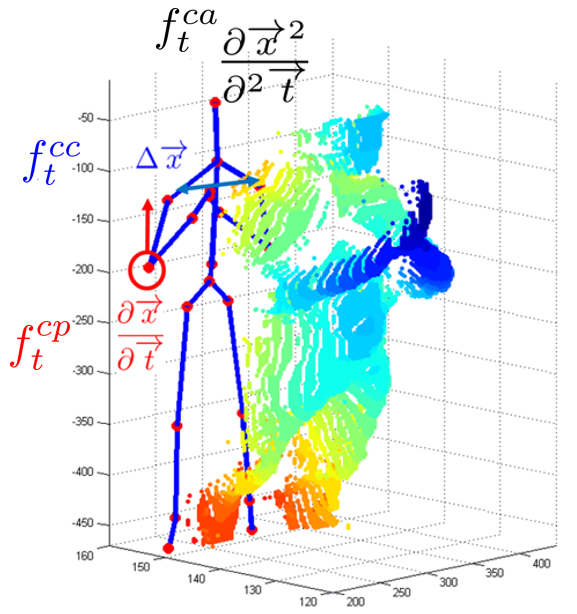
\includegraphics[width=0.3\textwidth]{images/point_cloud}\\
%  \caption{
%    A point cloud projection of a depth image and the 3D positional features.}
%    \label{point_cloud}
%\end{figure}
%
%
%\begin{figure}[t]
%  \centering
%  % Requires \usepackage{graphicx}
%  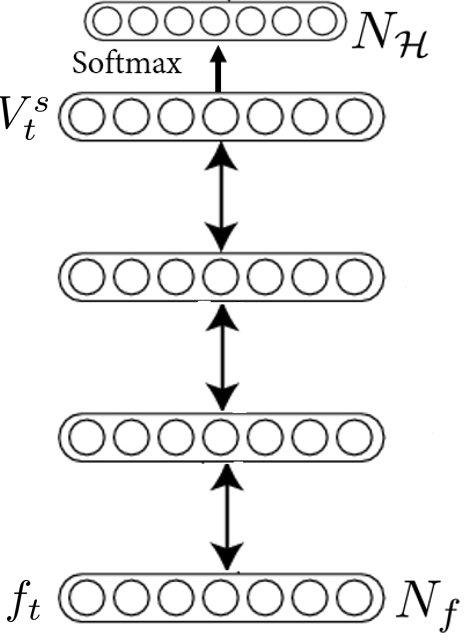
\includegraphics[width=0.23\textwidth]{images/DBN}\\
%  \caption{
%  A \DBN is trained to predict the emission probability  $p(\observationSK_t|\hiddenstate_t)$
%  from the  skeleton input \skfeature.
%  The double arrows indicate that the intermediate weights are first trained in an unsupervised fashion using stacked RBMs.
%}
%    \label{fig:DBN}
%\end{figure}


%\setlength{\fboxsep}{1pt}%
%\setlength{\fboxrule}{1pt}%
\begin{figure}[t]
       \centering
        \begin{subfigure}[c]{0.2\textwidth}
        \centering
                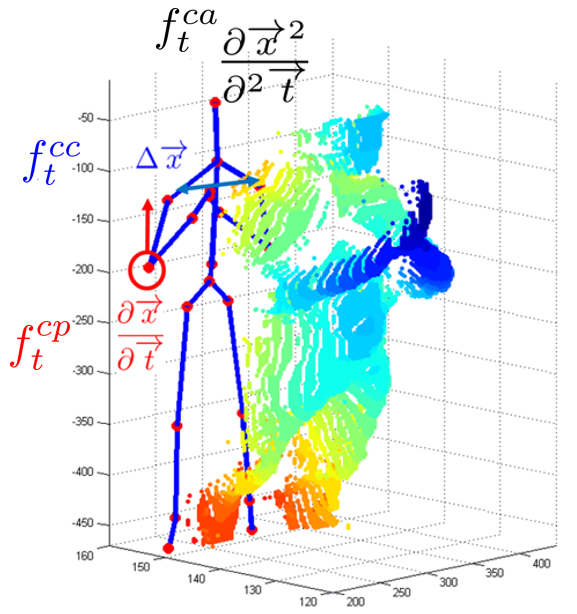
\includegraphics[width=4.5cm,height=5cm, clip]{images/point_cloud}
        \end{subfigure}%
        \hfill
        \begin{subfigure}[c]{0.2\textwidth}
        \centering
                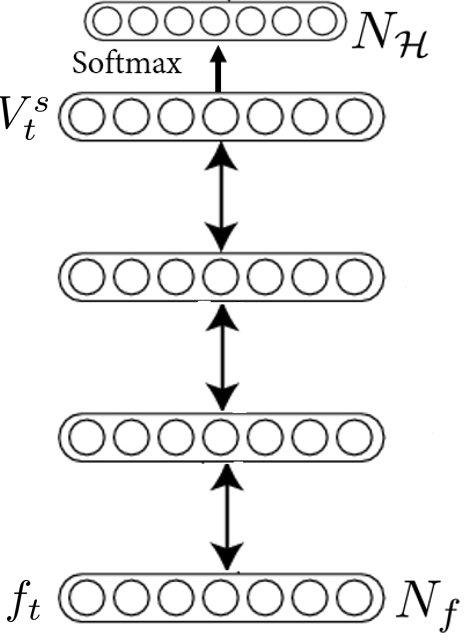
\includegraphics[width=4cm,height=5cm, clip]{images/DBN}
                %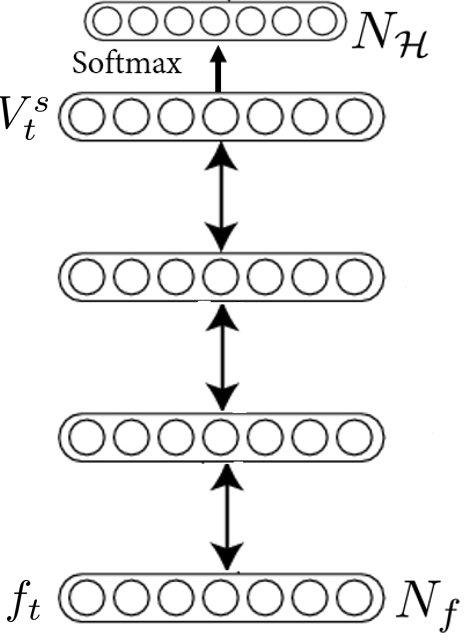
\includegraphics[width=0.2\textwidth]{images/DBN}
                %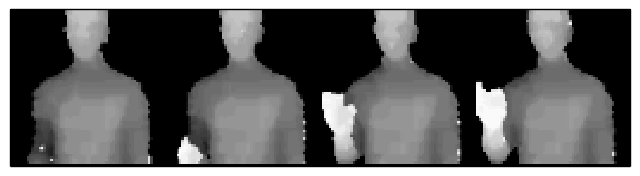
\includegraphics[width=2cm,height=3cm, trim=120 100 100 50, clip]{images/3dcnn_filters/original_images_depth_body_ok}
        \end{subfigure}
  \caption{
\small{ Left: A point cloud projection of a depth image and the 3D positional features.
  Right: A \DBN is trained to predict the emission probability  $p(\observationSK_t|\hiddenstate_t)$
  from the  skeleton input $\skfeature_t$.
  The double arrows indicate that the intermediate weights are first trained in an unsupervised fashion using stacked RBMs.
  }}
  \label{fig:DBN}\label{point_cloud}
\end{figure}


\subsubsection{Skeleton input features}

Given our task, only  the $\numberofjoints=11$ upper body joints are relevant and
considered, namely \emph{``ElbowLeft, WristLeft, ShoulderLeft, HandLeft, ElbowRight, WristRight, ShoulderRight, HandRight, Head, Spine, HipCenter"}.
%
The raw skeleton features of time $t$ are defined as $\skrawfeature_t=[\framefeature_t^{s,1}, \ldots, \framefeature_t^{s, \numberofjoints}]$.
To capture the gesture dynamics, rather than using $\skrawfeature_t$ as raw input to our data driven approach,
we follow the approach of~\cite{diwucvpr14} and compute the 3D positional pairwise differences of joints as well as temporal derivatives, defined as (as shown in Fig.~\ref{point_cloud}) \footnote{Note that the offset features used in~\cite{diwucvpr14} depend on the first frame.
Thus if the initialisation fails which is a very common scenario, the feature descriptor will be generally very noisy.
Hence, here we do not use these offset features.}:
\begin{align}
f^{cc}_t&=\{x_t^{s,i}-x_t^{s,j} | i,j=1,2,\ldots, N_j; i\neq j\} \label{sk_features_1}\\
f^{cp}_t&=\{x_{t+1}^{s,i}-x_t^{s,i} |  i=1,2,\ldots, N_j\} \label{sk_features_2}\\
f^{ca}_t&=\{x_{t+1}^{s,i} - 2 \times x_t^{s,i} + x_{t-1}^{s,i} | i=1,2,\ldots, N_j  \} \label{sk_features_3}
\end{align}
%
This results in an input feature vector $\skfeature_t=[f^{cc}_t, f^{cp}_t, f^{ca}_t]$ of dimension $N_{\skfeature}=N_j \times( \frac{ N_j}{2} + N_j + N_j)*\mathit{3}=891$.
Admittedly, here we do not completely neglect human prior knowledge about information extraction for relevant static postures, velocity and acceleration of overall dynamics of motion data.
While we have indeed used prior knowledge to define our relevant features, we believe they remain quite general and do not need dataset specific tuning.
Note that the feature extraction process resembles the computation of the
\emph{Mel Frequency Cepstral Coefficients (MFCCs)} and their temporal derivatives
typically used in the  speech recognition community~\cite{mohamed2012acoustic}.
%\textbf{\emph{Caveat}}:
%\begin{itemize}
%\item  When extracting skeletal features, the 3D joint coordinates have not been transformed from the world coordinate system to a person centric coordinate system by placing the \emph{``HipCenter"} at the origin.
%\item  Note also that the normalization scheme by scaling the skeleton position using length of \emph{``HipCenter"} and \emph{``Spine"} didn't work well in the implementation.
%\item The third point worth noting is that some actors performed gestures using left hand as a dominant hand whereas some using right hand which worth investigating the effect of this in the future. However, those tokens are treated indiscriminately.  Hence, the feature fed into \emph{GRBM} are almost raw, un-preprocessed.
%\end{itemize}

\subsubsection{Modeling \randomvariableSK{} using Deep Belief Networks}


%We briefly introduce the building elements of the network and a more detailed introduction can be found at:
%Boltzmann Machines (BMs) are a special structure of Markov Random Field (MRF), \emph{i.e.} the energy function is linear in term of its corresponding free parameters.
%To empower the expressiveness of the model so as to encode complex distributions, the hidden variables are introduced to enhance the modelling capability of the Boltzmann Machinesd with a two-layer structure, has the visible binary stochastic units $v\in \{0,1\}^D$ connected to the hidden binary stochastic units $h\in \{0,1\}^F$.
%
%The energy of the state $\{v,h\}$is:
%\begin{eqnarray}
%E(v,h;\theta)&=&-v ^{\top}Wh-b^{\top}v-a^{\top}h  \\
%             &=&-\sum^D_{i=1} \sum^F_{j=1} W_{ij} v_i h_j -\sum^D_{i=1}b_iv_i - \sum^F_{j=1}a_jh_j
%   \label{energy}
%\end{eqnarray}
%where $\theta=\{W,b,a\}$ are the free parameters: $W_{i,j}$ serves as the symmetric synergy term between visible unit $i$ and hidden unit $j$; $b_i$ is the bias term of the visible units and $a_j$ is the bias term of the hidden units.
%The joint distribution over the visible and hidden units is defined by:
%\begin{eqnarray}
%    P(v,h;\theta)&=&\frac{1}{Z(\theta)} \exp(-E(v,h;\theta)); \\
%        Z(\theta)&=&\sum_v \sum_h exp(-E(v,h;\theta))
%    \label{RBM}
%\end{eqnarray}
%The conditional distributions needed for inference and generation are given by:
%\begin{eqnarray}
%    P(h_{j=1}|\textbf{v})&=&g(\sum_i W_{ij}v_i+a_j)); \\
%      P(v_{i=1}|\textbf{h})&=&g(\sum_j W_{ij}h_j+b_i))
%\end{eqnarray}
%where $g(x)=\frac{1}{1+exp(-x)}$ is the logistic function.

%The derivative of the log-likelihood with respect to the model parameter from Eq.~\ref{RBM} is expressed as: $E_{P_{data}}[vh^{\top}]-E_{P_{model}}[vh^{\top}]$ where $E$ denotes the expectation.
%Due to the intractability of the second term, an approximation is generally required. This approximation is called the ``Constrative Divergence":
%%In practice, learning is done by following an approximation to the gradient of a different objective function, called the ``Constrative Divergence":
%\begin{equation}
%    \Delta W = \alpha (E_{P_{data}}  [\textbf{vh}^T]-E_{P_T}[\textbf{vh}^T]). \label{CD1}
%\end{equation}
%where $\alpha$ is the learning rate and $P_T$ is the distribution obtained by running a Gibbs chain, initialized with the visible units given by the data, for $T$ full steps.

Given the input skeleton feature \skfeature, a \DBN model is used to predict the emission probability, as shown in Fig.~\ref{fig:DBN}.
As explained in Section~\ref{sec:emissionprob}, the learning proceeds in two steps:
in the first one, the network is considered as a stack of RBMs, and trained using a greedy, layer-by-layer
unsupervised learning algorithm \cite{hinton2006fast};
in the second one, a softmax network layer is added on top of the RBMs to create a \DBN architecture,
where the  weights of the first step are used to initialize the corresponding weights in the \DBN,
and the \DBN is further trained and fine-tuned in a supervised fashion to predict the emission probability.
%
The number of nodes at each layer of the \DBN are $[N_{\skfeature},2000,2000,1000,\numberhiddenstate]$.
% where $N_f = 891$ is the observation domain dimensionality; $N_{\mathcal{H}}$ is the output target class.
We provide below further details on the model and training.

\mypartitle{Gaussian-Bernoulli RBM.}
%
Restriced Boltzmann machine (RBM) are undirected graphical models involving visible and hidden variables,
with symmetric connections between the hidden and visible units but no connection within hidden variables
or visible variables.
%
In most cases, RBMs rely on binary random variables.
%
However, in our case the visible unit in the first layer are the vector of skeleton features $\skfeature \in \mbf{R}^{N_{\skfeature}}$, which are continous.
To account for this situation, we thus resort to a Gaussian-Bernoulli RBM (\emph{GRBM})~\cite{salakhutdinov2009learning},
whose main difference w.r.t. standard RBM lies in the following:
the energy term of our first layer $\skfeature$ to the hidden binary stochastic units $\rbmh \in \{0,1\}^F$ is given by:
\begin{equation}
    E(\skfeature,\rbmh;\theta) =-\sum_{i} \frac{(\skfeatureel_i-b_i)^2}{2\sigma_i^2} -\sum_{i} \sum_{j} W_{ij}  \rbmhel_j \frac{\skfeatureel_i}{\sigma_i}- \sum_{j=1}a_j\rbmhel_j
\label{GRBMenergy}
\end{equation}
where $\theta=\{W,b,a\}$ are the free parameters: $W_{i,j}$ serves as the symmetric synergy term between visible unit $i$ and hidden unit $j$,
while $b_i$ and $a_j$ are the bias term of the visible and hidden units, respectively.
%
The conditional distributions needed for inference and generation are given by the traditional logistic function $g$ for the binary hidden variable, and the normal distribution $\mathscr{N}$  for the continous variable:
\begin{eqnarray}
    P(\rbmhel_j=1 | \skfeature) & = & g (\sum_i W_{ij} \skfeatureel_i+a_j) \\
    P(\skfeatureel_i=\skfeatureel|\rbmh) & = & \mathscr{N}( \skfeatureel |\mu_i,\sigma_i^2).
\end{eqnarray}
where $\mu_i=b_i+\sigma_i^2 \sum_j W_{ij}$.
In practice, we normalise the data (mean substraction and standard deviation division) in the preprocessing phase.
Hence, instead of learning $\sigma_i^2$, one typically used  $\sigma_i^2=1$ during training.

We ran 100 epochs using a fixed recipe based on stochastic gradient descent with a mini-batch size of 200 training cases
to train  the stacked RBM, in which the learning rate is fixed at 0.001 for the Gaussian-Bernoulli RBMs,
and at 0.01 for the following binary-binary RBMs.






\mypartitle{\DBN forward training.}
%
% In the training set, there are in total $400\,117$ frames. During the training of the \emph{DBN}, $90\%$ is used for training, $8\%$ for validation (for the purpose of early stopping) $2\%$ is used for test evaluation.
%
The \DBN is initialized with the result of the previous step, a method which tends to avoid suboptimal local minima and increase
the network’s performance stability.
%
The learning rate for the parameter fine tuning
starts at 1 with 0.99999 mini-batch scaling. During the experiments, early stopping occurs around epoch 440.
The optimisation completes with a frame based validation error rate of $16.5\%$.%, as shown in  Fig~\ref{sk_error_rate}.

% Although that further optimising the network architecture would lead to more competitive results, in order not to overfit, ``as algorithms over time become too adapted to the data set, essentially memorising all its idiosyncrasies, and losing ability to generalise"~\cite{torralba2011unbiased}, we would like to treat the model as the aforementioned more generic approach.
% Since a completely new approach will initially have a hard time competing against established, carefully fine-tuned methods.
%More fundamentally, it may be that the right way to treat dataset performance numbers is not as a competition for the top place.
%This way, fundamentally new approaches will not be forced to compete for top performance right away, but will have a chance to develop and mature.
%The performance of the skeleton module is shown in Tab.~\ref{Table_score_fusion}.

%\begin{figure}[t]
%  \centering
%  % Requires \usepackage{graphicx}
%  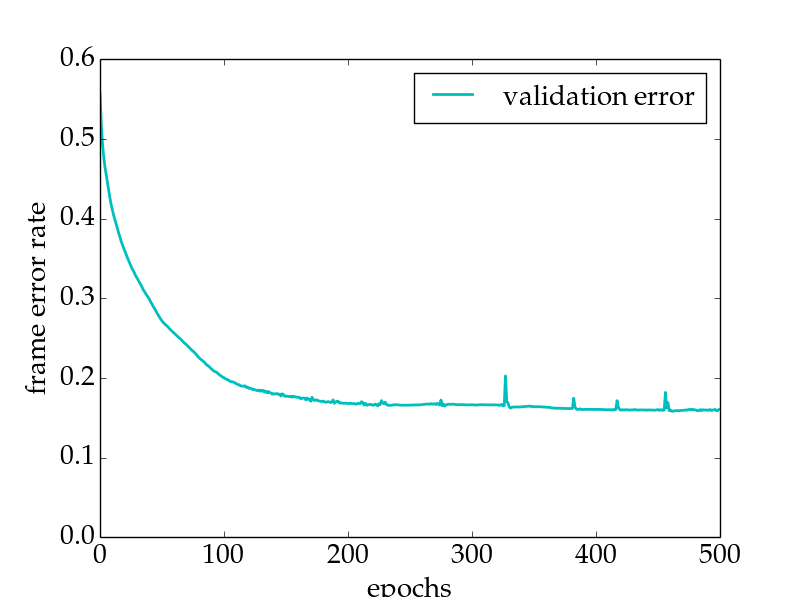
\includegraphics[width=0.4\textwidth]{images/sk_training_error}\\
%  \caption{
%    \small{Deep Belief Network frame based validation error rate for the skeleton modality.}
%%    The 0.05 frame error rate indicates the good generalisation property of the DBN skeleton module.
%    }
%    \label{sk_error_rate}
%\end{figure}

\subsection{RGB \& Depth 3D Module} \label{sec:rgbd_modules}
\subsubsection{Preprocessing}\label{3d_preproc}
\begin{figure*}[t]
  \centering
  % Requires \usepackage{graphicx}
  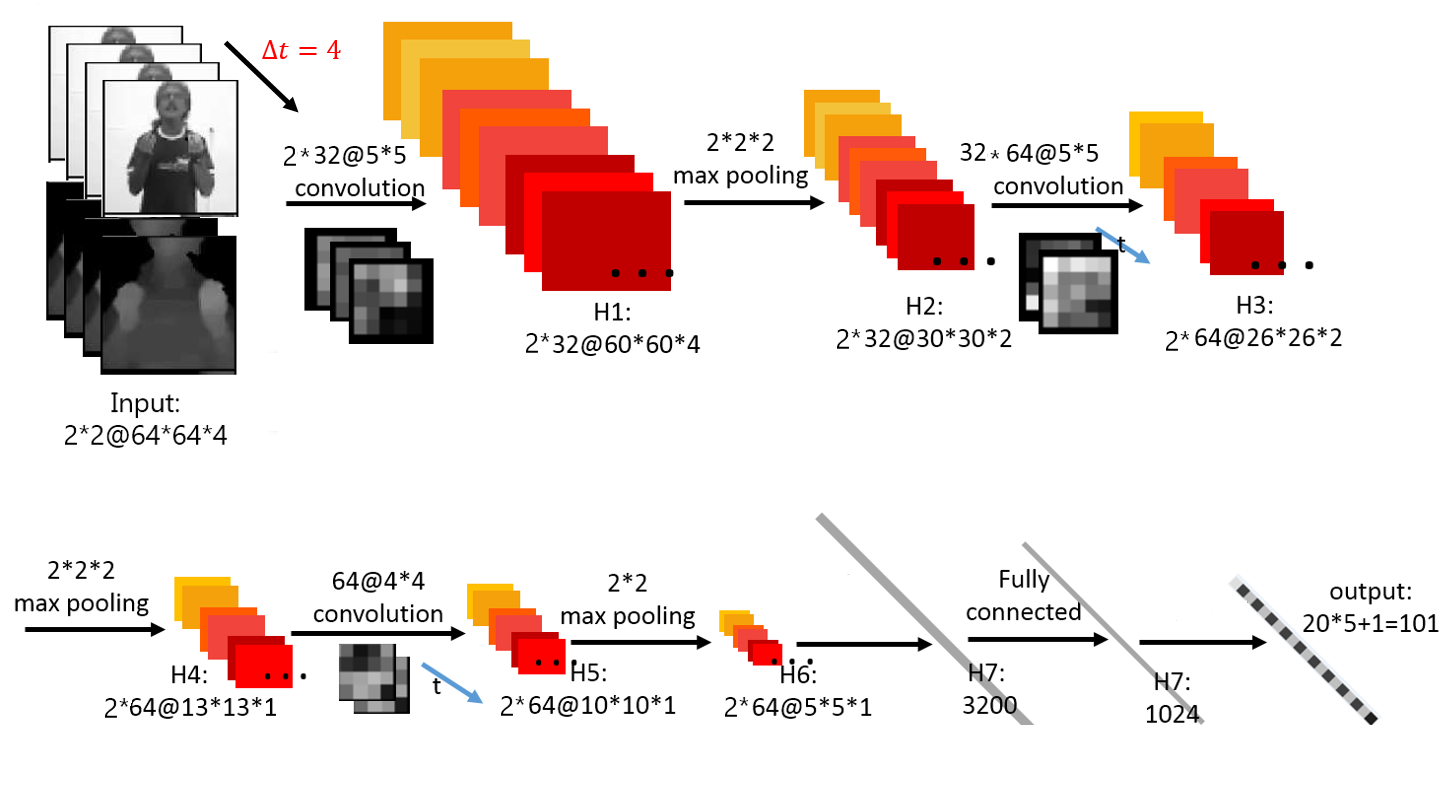
\includegraphics[width=.9\textwidth]{images/3DCNN_new}
\vspace*{-2mm}
  \caption{3DCNN architecture. The input is $2\times2@64\ast64\ast4$, meaning 2 modalities (depth and RGB)  for the hand and body regions,
each  being 4  consecutive 64 by 64 frames stacked together. See text for further details.
%
%Note that in H1, the Depth and RGB  response maps of the hand (and body) are summed to produce a single feature map,
%while in H7, the hand and body part feature maps of H6 are just flattened.
}
\label{3dcnn_architecture}
\end{figure*}
Although DeepMind technology~\cite{mnih2013playing} presented the first deep learning model to successfully learn control policies directly from high-dimensional sensory input using deep reinforcement learning, working directly with raw input Kinect recorded data frames, which are $640 \times 480$ pixel images, can be computationally demanding.
Therefore, our first step in the preprocessing stage consists of cropping the highest hand and the upper body using the given joint information. In the Chalearn dataset, we determined that the highest hand is the most interesting. When both hands are used, they normally perform the same (mirrored) movement, and when one hand is used, it is always the highest one which is relevant.
Furthermore, to be invariant to handedness, we always train the model with the right hand view.
That is, when the left hand is actually the performing hand, the video was mirrored.


The preprocessing results in four video samples (body and hand with grayscale and depth) of resolution $64\times64$.
Furthermore, the noise in the depth maps is reduced by removing the background using the automatically produced
segmentation mask provided with the data, and applying a  median filtering.
%
Depth images are Z-normalised (the mean is subtracted -as it is rather irrelevant to the gesture subclass-
and the result divided by the standard deviation), whereas
RGB images are only normalized by the image standard deviation.
The outcome is illustrated in Fig.~\ref{3dcnn_filters}.
%\begin{figure}[t]
%  \centering
%  % Requires \usepackage{graphicx}
%  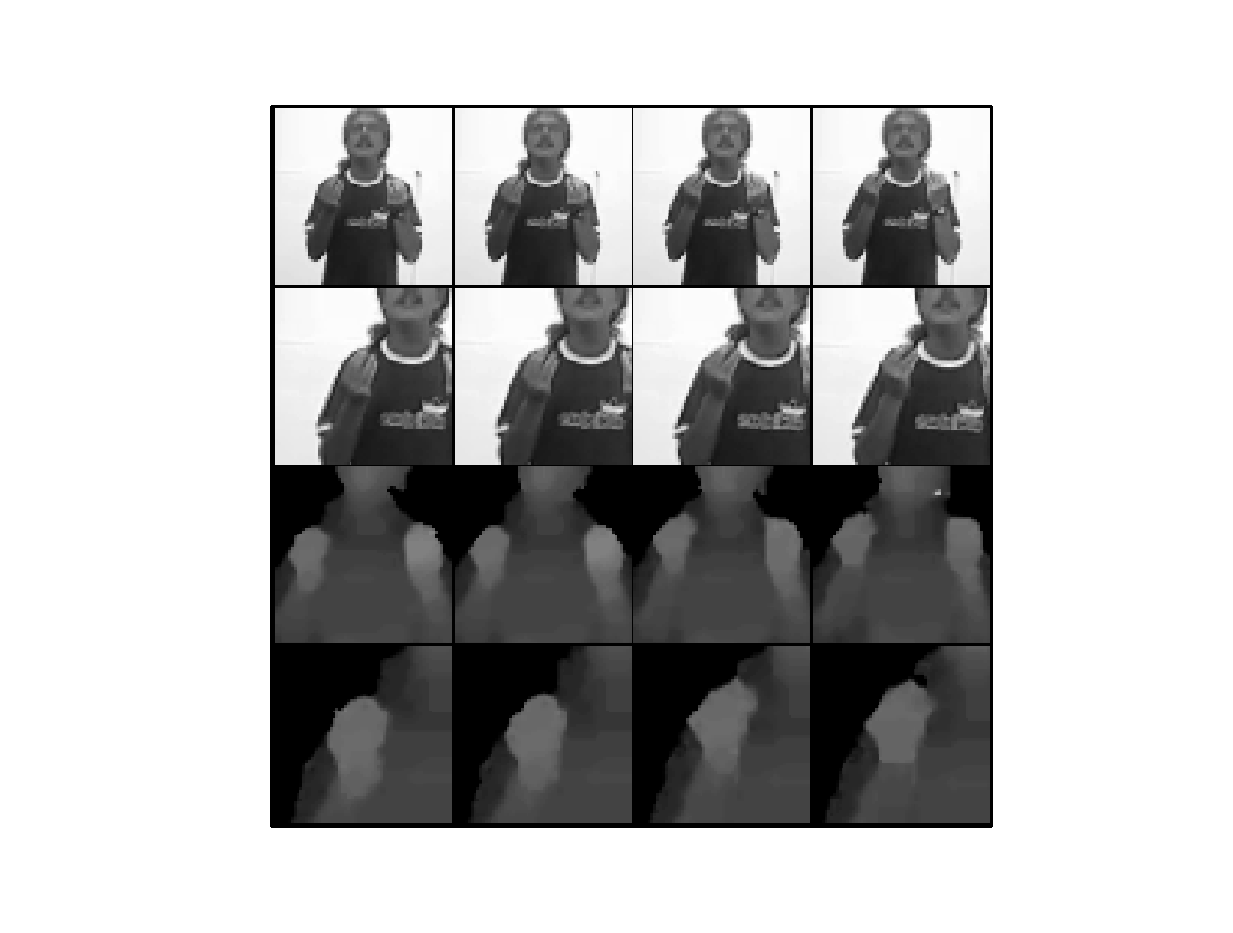
\includegraphics[width=0.5\textwidth]{images/3dcnn_filters/original.eps}\\
%  \caption{
%    Preprocessing result. Inputs  from top to bottom: 1) grayscale body input, 2) grayscale hand input, 3) depth body input, 4) depth hand input. }
%    \label{3dcnn input}
%\end{figure}


\subsubsection{3DCNN Architecture}
\label{sec:3dcnnArchitecture}

This  architecture consists of a series of layers composed of either convolution, pooling or, in the last layer, fully connected layers.
The 3D convolution itself is achieved by convolving a 3D kernel to the cuboid formed by stacking multiple contiguous frames together.
We follow the nomenclature of in~\cite{ji20133d}.
However, instead of using $tanh$ units~\cite{ji20133d},  Rectified Linear Units (\emph{ReLUs})~\cite{krizhevsky2012imagenet}
were used in order to speed up training.
Formally, the value of a unit at position $(x, y, z)$ ($z$ here corresponds to the time-axis) in the $j$-th feature map in the $i$-th layer, denoted as $v^{xyz}_{ij}$, is given by:
\begin{equation}
v^{xyz}_{ij} =  max( 0,  ( b_{ij} + \sum_m \sum_{p=0}^{P_i - 1} \sum_{q=0}^{Q_i -1 } \sum_{r=0}^{R_i -1} w^{pqr}_{ijm} v^{(x+p)(y+q)(t+r)}_{(i-1)m} ))
\label{ReLU}
\end{equation}
%
The complete 3DCNN architecture is depicted in Fig.~\ref{3dcnn_architecture}:
4 types of input contextual frames are stacked as size $64\times64\times4$ (as illustrated in Fig.~\ref{3dcnn_filters}).
%
The first layer (H1) consists of 32 feature maps produced by $5\times5$ spatial convolutional kernels,
followed by local contrast normalisation (LCN)~\cite{jarrett2009best}.
%
Note that the filter response maps of the Depth and RGB images of the hand (and body) are summed to produce a single feature map,
thus resulting in H1 in 32 feature maps for each of the hand and for the body region.
%
A 3D max pooling with strides $(2,2,2)$ is then applied.
%
The second layer uses 64 feature maps with $5\times5$ kernels followed by LCN and 3D max pooling with strides $(2,2,2)$.
The third layer is composed of 64 feature maps with $4\times4$ kernels followed by 3D max pooling with strides $(1,2,2)$.
All hand and body convolutional layer outputs of H6 are flattened in H7, and fed into one fully connected layer of size $1024$.
%
Finally, the output layer has \numberhiddenstate values, the number of states in the HMM state diagram (see Fig.~\ref{HMM_ES}).




\subsubsection{Details of Learning}
% The first 650 batches are used for training and the remaining 50 files for validation.
During training, dropout \cite{hinton2012improving} is used as main regularisation approach to reduce overfitting.
Nesterov’s accelerated gradient descent (NAG) \cite{sutskever2013importance} with a fixed momentum-coefficient of 0.9 and mini-batches of size 64 are also used.
The learning rate is initialised at 0.003 with a 5\% decrease after each epoch. The weights of the 3DCNNs are randomly initialised with a normal distribution with $\mu = 0$ and $\sigma = 0.04$.
The frame based validation error rate is $39.06\%$ after 40 epochs. % as shown in Fig.~\ref{fig:RGBErrorRate}.
Compared with the skeleton module (16.5\% validation error rate), the 3DCNN has a notable higher frame based error rate.


%\begin{figure}[t]
%  \centering
%  % Requires \usepackage{graphicx}
%  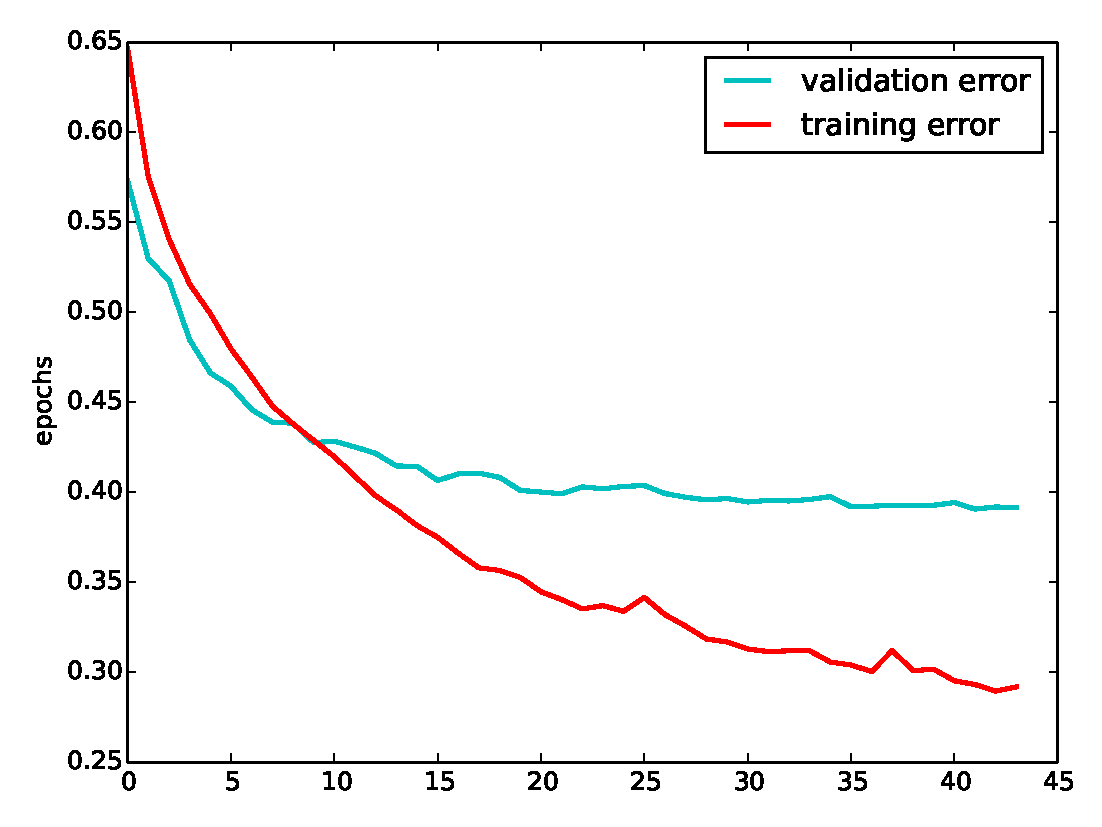
\includegraphics[width=.4\textwidth]{images/3dcnn_filters/training_error}
%  \caption{
%  \small{Frame based error rate of the 3DCNN.
% The error rates are much higher than when using the skeleton module (see Fig.~\ref{sk_error_rate})
% indicating that  learning from images is more difficult. }}
%\label{fig:RGBErrorRate}
%\end{figure}

\subsubsection{Looking into the Networks: visualisation of Filter Banks}

The convolutional filter weights of the first layer are depicted in Fig.~\ref{3dcnn_filters}.
The unique characteristics from the kernels are clearly visible: as hand input images (RGB and depth) have larger homogenous areas
than the body inputs, the resulting filters are smoother than their body counterpart.
In addition, while being smoother overall than the grayscale filters, depth filters exhibit stronger edges,
as also reported in~\cite{socher2012convolutional}.
%
Finally, by looking at the joint depth-image response maps, we can notice that some filters better capture segmentation like information,
while other are more edge oriented.

\begin{figure*}[t]
  \centering
  % Requires \usepackage{graphicx}
  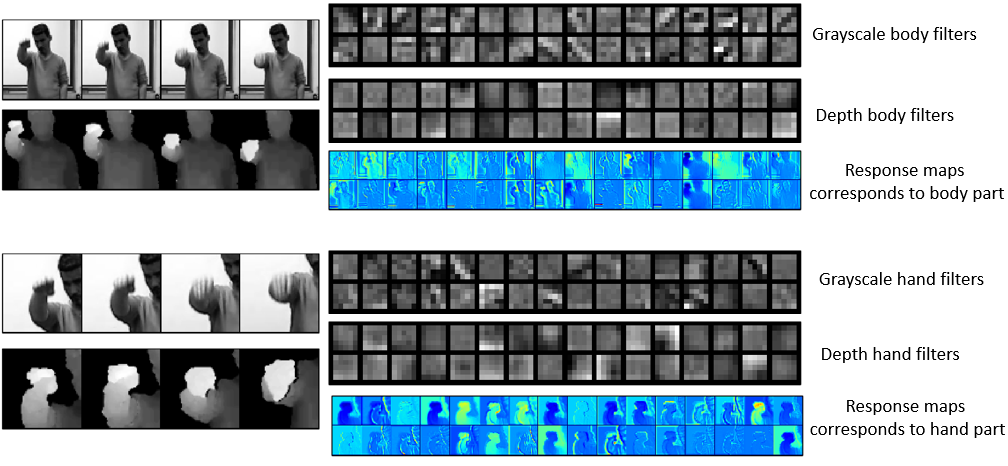
\includegraphics[width=0.85\textwidth]{images/CNN_filters}
  \caption{
  \small{Visualisation of input frames, first convolutional layer $5\times5$ filters, and corresponding response maps.
As depth images are smoother than the grayscale ones, the corresponding filter are smoother as well.}
}\label{3dcnn_filters}
\end{figure*}


\subsection{Multimodal Fusion}
To combine the two modalities, two strategies can be used, as shown in Fig.~\ref{fig:fusion}:
a late fusion approach and an intermediate fusion approach.


\subsubsection{Late Fusion}
%
This scheme fuses the combination of the emission probabilities estimated from the different input.
While different combination schemes exist, here we considered a simple linear combination:

\begin{equation}
\emissionprob  \propto  \alpha \cdot  \emissionprobSK + (1-\alpha)\cdot  \emissionprobRGBD
\end{equation}
where the different emission probabilities are provided by the modules described in \ref{sec:skeleton_module} and \ref{sec:rgbd_modules},
and $\alpha$ is a coefficient that controls the contributions of each source of information and which is estimated by cross validation.
Interestingly, the best performing $\alpha$ is close to $0.5$, indicating that both modalities are equally important.


\subsubsection{Intermediate Fusion}
\label{early_fusion}

As an alternative to the late fusion scheme, we can take advantage of the high-level representation implicitly learned by each module
(and represented by the \highSK and \highRGBD nodes of the penultimate layer of the respective networks, before the softmax)
to fuse the modality in an intermediate fashion by concatenating these two layers in one layer of 2024 hidden unites
and learning a cross-modality emission probability predictive network.
%
Note that this is very similar in spirit to the approach proposed in \cite{Ngiam2011multimodal}
for audio-visual speech recognition.
%
An important difference is that in \cite{Ngiam2011multimodal}, the same stacked RBMs/\DBN architecture was used
to represent both modalities before fusion, whereas in our case, a stacked RBMs/\DBN and a \ThreeDCNN are used.
%
Also, \cite{Ngiam2011multimodal} proposed the use of a multimodal autoencoder to handle predictions when potentially
only one modality migth be present, a point that we do not address.

The resulting architecture is trained by first initializing the weights of the deeper layers from the previously trained module,
and then jointly fine tuning the whole network (including learning the last layer parameters).
The training is stopped when the validation error rate stops decreasing ($\sim$15 epochs).
%
We argue that using the ``pre-trained" parameters is important due to the heterogeneity of the inputs of the system,
and that the joint training should adjust parameters to handle  this heterogeneity and produce the final estimates.


\begin{figure}[t]
  \centering
  % Requires \usepackage{graphicx}
  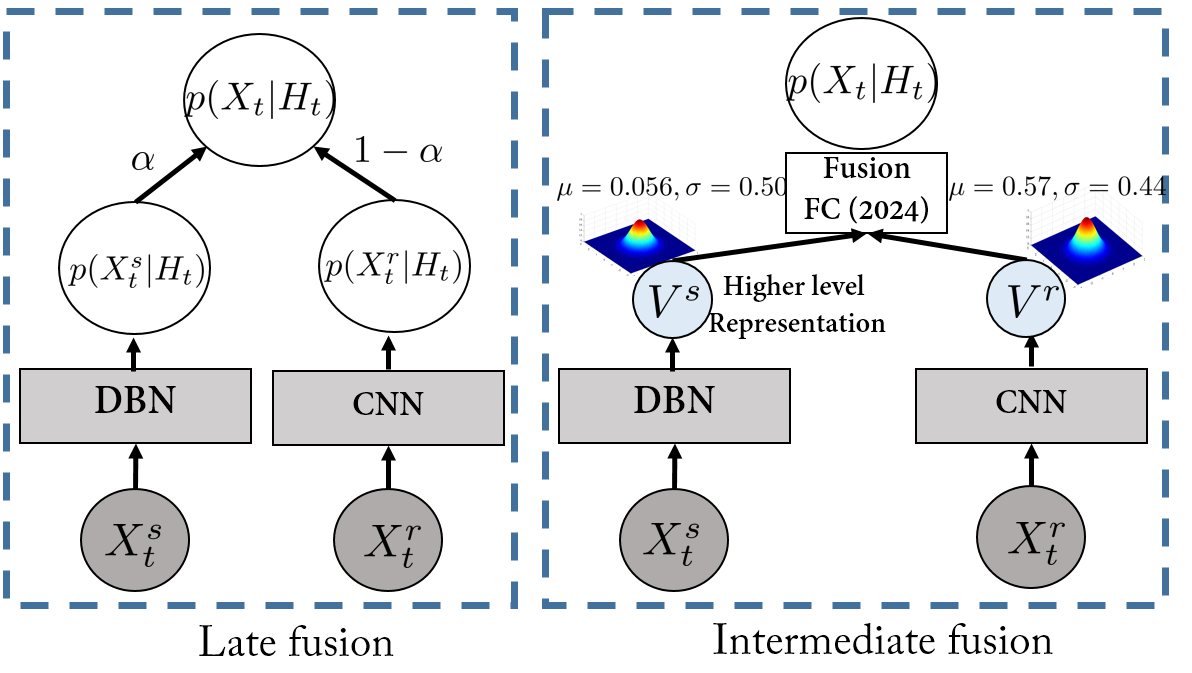
\includegraphics[width=0.5\textwidth]{images/Fusion_combined}
\vspace*{-2mm}
\caption{
\small{
Multimodal dynamic networks with late fusion scheme (left) and intermediate fusion scheme (right).
The late approach simply combines the emission probabilities from two modalities.
In the intermediate fusion scheme, each modality (skeleton and \RGBD) is first pre-trained separately,
and their high-level representation \highSK and \highRGBD (the penultimate node layers of their neural networks)
are concatenated to generate a shared representation. The resulting architecture is trained jointly.}
  }\label{fig:fusion}
\end{figure}



\endinput
